\documentclass[fleqn,10pt,lineno]{wlpeerj}

\title{Additional details on functional boxplots \ali{a better title?}}

\author[1]{Ali Gharouni}
\author[1,2,3]{Benjamin M. Bolker}
\affil[1]{Department of Mathematics \& Statistics, McMaster University, Hamilton, Canada}
\affil[2]{Department of Biology, McMaster University, Hamilton, Canada}
\affil[3]{Michael G. DeGroote Institute for Infectious Disease Research, McMaster University, Hamilton, Canada}
\corrauthor[1]{First Author}{agharoun@uottawa.ca}

% \keywords{Functional depth, Functional boxplot, Centroid}

\begin{abstract}
This is a commentary work motivated by Juul et al. (2021)’s work in which a few useful ideas
of the concept of the central set out of an ensemble of epidemic curves were presented. In the present work we provide an alternative, and more principled, curved-based statistics approaches to approximate the most central set which represents the central 90\% of the ensemble. In particular, we use two functional ranking methods; (1) the sampling-based, fast and robust functional boxplot, and (2) a multivariate generalization of ranking the curves by using Mahalanobis distance among features of interest. We apply our methods on Juul et al. (2021)’s dataset and compare our results with theirs.
\end{abstract}

\begin{document}

\flushbottom
\maketitle
\thispagestyle{empty}

\section*{Introduction}

Developing robust and computationally efficient inference tools for ensembles of curves -- functional data in general -- is necessary to summarize features of interest and study the uncertainty. These tools are even more important when it is about accuracy in forcasting trajectory of epidemic curves produced form different models which may vary from deterministic, stochastic to the individual-based models. Fixed-time descriptive approaches (e.g., computing pointwise quantiles) have been classically used (see, for example, \citep{ferguson2005strategies,chinazzi2020effect}). 
\cite{juul2021fixed} pointed out shortcomings to the standard ways that researchers draw confidence intervals for ensembles of curves, with specific examples drawn from the output of stochastic epidemic models. In particular, they showed that fixed-time approaches can fail to capture the uncertainty in key features of an epidemic such as the timing and magnitude of epidemic peaks. As an alternative to fixed-time approaches, the authors illustrated methods to compute the \emph{central set} of an ensemble of curves, a high-dimensional analogue of interquartile range or confidence interval. There is also a large body of literature on this topic under the rubrics of \emph{functional depth} and \emph{functional boxplots} for high dimensional data which we review briefly.

The concepts of order statistics and ranks for univariate data enable one to estimate the most central region,  i.e., interquartile range, the sample mean and sample median. In multivariate setting, these concepts have been generalized to the concept of depth with several definitions \citep{mahalanobis1936generalized, tukey1975mathematics, oja1983descriptive, liu1990notion, singh1991notion, vardi2000multivariate, zuo2003projection}. Functional depth was proposed by \cite{fraiman2001trimmed} as the integral of univariate $L_1$-depths developed by \cite{vardi2000multivariate}.
\cite{lopez2007depth} developed functional band depth (FBD) which is a sample-based method for determining a curve's centrality (and hence whether it should be included in a central set of curves for display). It measures the fraction of times that a given curve is completely included within the envelope of a set of other curves randomly sampled from the ensemble. The sample size is determined by a \emph{tuning parameter} denoted by $J$, and the number of samples is determined by all possible combinations. As the next canonical extention, functional boxplot was developed based on functional depth to display the data, highlight their characteristic, and reveal interesting features \citep{sun2011functional,sun2012exact}. \cite{wynne2021statistical} used a machine learning approache -- specifically, kernel mean embedding -- to study the functional depth.

In a comparable approach to FBD algorithm, \juul primarily studied the curve centrality on an epidemic ensemble. They chose the \emph{tuning parameter} as $J=50$ (they use the notation \ncurve), and chose $\nsample=100$ such samples to compute the fraction (\emph{band depth}) for each curve. They provided open-source Python code that implements this method, as well as some of the weighted variants they discuss. For the simple (unweighted) case, however, there are already mature open source implementations available in R \citep{fda_pkg,roahd}, Matlab (\url{https://www.psych.mcgill.ca/misc/fda/downloads/FDAfuns/}), and Python \citep{seabold2010statsmodels}. In general these packages use the same functional band depth measure as \juul, but substituting $J=2$, which is robust \citep{lopez2009concept} and allows the use of a computationally efficient algorithm for large data sets \citep{sun2012exact}. It is unclear why \juul chose larger values of $J$ (10 and 50), although the dimensions of their examples are small enough that the computational burden is not important.

\juul also suggest ranking according to a single, one-dimensional feature of interest such as the maximum values of newly hospitalized cases in a single day (their Fig.~2e). We suggest that this approach could be extended to incorporate multiple features of interest. Functional band depth could again be used on this reduced set of features; here we use the \emph{Mahalanobis distance} \citep{mahalanobis1936generalized}, which measures distance from a centroid accounting both for variation in the scales or typical magnitudes of different features and for correlation among features.
Our example uses a feature set including the peak value of incidence (new infections), the time at which the peak occurs, and the initial growth rate, duration, and final size of the epidemic. While these are typical epidemiological features of interest, researchers can and should choose the features that are most closely connected to their particular research questions \citep{probert2016decision}.

In this work, we explore \juul curve-based statistical approach in more depth which led us to several useful practical and theoretical points that could be useful for researchers interested in using these approaches. In particular, we compare the following methods for determining a curve's centrality on the epidemic ensemble provided in \juul's work; (i) \juul's primary sampling-based method (ii) the functional band depth measure (FBD), and (iii) ranking the curves by using Mahalanobis distance among features of interest.

\section*{Methods}

In our exploration, we present the comparison of 90\% central regions computed with different functional boxplot methods.
First, we implemented \juul's primary sampling-based method in R \citep{R} for determining a curve's centrality which in nature is similar to FBD with minor differences in sample size and number of samples. In particular, the implemented algorithm involves the following steps. (i) a subset of curves was randomly sample from the ensemble (FBD: J=2, \juul : J=50), (ii) compute the sample-specific min-max envelopes, (iii) score individual curves based on whether they lie entirely within the envelope (thus, score=1) or not (thus, score=0), and (vi) repeat to derive a centrality scoring or "rank" on [0,1] for each curve based on the proportion. In particular, the curve-specific rank is estimated by the 'median-like' criterion (sumation of scores). In order to characterize and plot the "central region", we assume that the most central curves are the ones with their ranks > 0.1 quantile to get 90\% central region. 

Secondly, we used the function fda() in R \citep{R} package \pkg{roahd} \citep{roahd}, with the choice of modified band depth (MBD) to break ties which is based on the fast algorithm proposed by \cite{sun2012exact}. Likewise the implemented method, the curve-specific ranks are sorted and the "central" region was ploted. 

Thirdly, for an individual curve in the ensemble, a feature vector was assigned. The curves are ranked according to thier feature vector. Specifically, we used function mahalanobis() in R \citep{R} to compute the pairwise Mahalanobis distance between the features of two curves with the covariance matrix from the entire data set as the scaling factor. This is because we can't compute the covariance matrix for only two samples. In this case, the rank of each curve is the average distance to the rest of the set. The 90\% central region is considered as curves with ranks < 0.9 quantile. Note that, the following features of interest were chosen for each curve in the ensemble; (i) the peak value of incidence (new infections), (ii) the time at which the peak occurs, (iii) the initial growth rate, (iv) epidemic duration, and (v) final size of the epidemic. Specifically, the peak was determined by the global maximum of a curve on its domain. The initial growth rate was estimated by fitting an exponential function to the section of the curve starting from the first day of nonzero prevalence to the day when the prevalence is 10\%. The epidemic duration was determinded by the time between 10\% and 90\% prevalence cumulative cases. The final size was given by the integration of the curve over time.




\section*{Results}

\begin{figure}[ht]\centering
  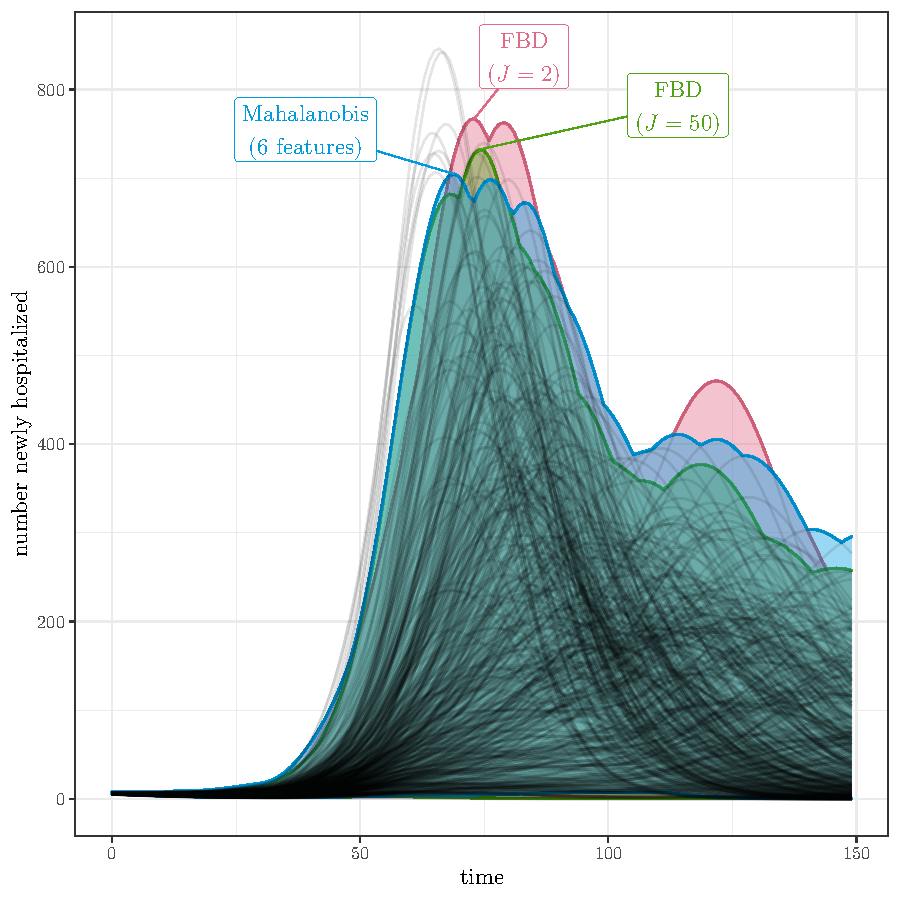
\includegraphics[width=\linewidth]{scripts/cent_plot.pdf}
  \caption{Comparison of 90\% central regions computed with
    different functional boxplot methods, using epidemic curve ensembles from \juul. FBD = functional band distance; $J$ = number of curves used for centrality calculation. Curve with $J=2$ computed via the \texttt{roahd} package \citep{roahd}: curve with $J=50$ used our own implementation of the functional band distance algorithm described by \juul.
  }
  \label{p.a}
\end{figure}
 
\section*{Discussion}

% this is discussion:
% While \juul do cite this literature \citep{sun2011functional}, exploring it in more depth led us to several useful practical and theoretical points that could be useful for researchers interested in using these approaches. 


We note that one potential problem with Mahalanobis distances is if (for example) the feature distribution is strongly bimodal, then scaling factors/correlations derived from the overall data set may not be appropriate for scaling the components of distance between two trajectories whose features put them in the same mode/component of the distribution.

\section*{Conclusions}

\section*{Acknowledgments}

\bibliography{./curveBP}
\end{document}